
\subsection{ParLOT vs.~Callgrind}
ParLOT can capture the function calls and returns at two major levels: 1) \textit{Main}, where it only traces the functions of the main image and 2) \textit{All}, which includes all library functions as well.

In this subsection, we compare the overhead of ParLOT(main) and ParLOT(all) with Callgrind, which is the most similar tool that we could find.
However, Callgrind does not use any significant compression (except for the name of functions) and stores the trace files in ASCII format. It only records enough information to produce the dynamic call graph and only for the main image, which may not be sufficient for finding the root cause of a failure since it might happen at lower levels or not be reflected in the call graph.
Fig.\ref{sd.pin.cg} and table \ref{t_sd.pin.cg} show the runtime normalized to the native runtime for different NAS apps and different configurations .
It seems that Callgrind has better results on larger number of cores but overall, the geomean of average slowdowns for both ParLOT(main) (1.56) and ParLOT(all) (1.63) is smaller than Callgrind (5.51).

Fig \ref{ts} and table \ref{t_ts} shows the required bandwidth for traces per core for ParLOT next to Callgrind.
The average trace bandwidth per core is less than 4 kB for ParLOT and is more 10 kB for Callgrind. Considering that Callgrind applies very poor compression of traces, ParLOT's maximum compression ratio of 13K (table \ref{t_compRatio},  shows the capability of ParLOT to store almost 50 MB worth of data in just 4 kB per core per second. The story becomes more impressive when you think about running any application on hundreds of cores and running ParLOT on top of that with smaller overhead than Callgrind but more sophisticated, informative and useful.
More importantly, 4 kB per core should be no problem for the local file system to handle and leaves most of the bandwidth for the application.

\subsection{Overheads}
The overall overhead adds to the original application due to instrumentation and tracing is a product of pure Pin overheaad, instrumentation, recording traces, compression and storing data(I/O).
In this section, we show the results of a set of experiments with disabling some or all features of ParLOT to see how much impact each component (fig \ref{overview}) has on the final overhead.
We categorized the overall overhead added to the native application into 1) pure overhead by Pin, 2) overhead by tracing (with and without compression) and 3) I/O overhead\\
We designed these variations of ParLOT to extract detailed overhead added by each category:
\begin{itemize}
\item \textbf{npin}: Every phase of ParLOT is disabled except Pin-Init (fig \ref{overview}) in \textit{npin} and it shows the pure overhead added by Pin. 
\item \textbf{wpin}: Compression is disabled in \textit{wpin} and all collected data would be stored as is to the disk. The results of this tools shows how much efficiency our compression approach adds to ParLOT. 
\item \textbf{dpin}: It is almost identical to ParLOT except it stores the generated compressed traces to "/dev/null". The purpose of \textit{dpin} is to see how much of the overall overhead is because of I/O.
\end{itemize}

Last row of the table \ref{t_overhead} shows the average overhead that each of above testing tools adds to the native execution. For each configuration, the differences between the average slowdown of dpin and pin is very insignificant which shows that ParLOT is not an I/O-bounded tool. 
Capturing, collecting and storing the data using ParLOT but without any compression, would cause up to more than 130X slowdown. Again it is another proof for the efficiency that our compression method within ParLOT provides for tracing.

Table \ref{} shows how much overhead each factor in the rows adds to the execution during PatLOT process.The smallest impact belongs to I/O.

\subsection{Compression Ratio and required bandwidth}

As we discussed in section ??, full function-call-invocation trace at granularity of library function calls, can help us gain information about the general control flow of the application to the point to detect bug manifestation and finding the root cause of the bug.
Our experiments shows that ParLOT compression algorithm can compress this type of information with high compression ratio up to 16k on average. 

Table \ref{t-compRatio} shows the average compression ratio. 





This table shows the average ParLOT compression ratios for different NAS applications from the generated traces. For column \textbf{ep} the ratio is high up to 16k.



\textbf{npin}: Every phase of ParLOT is disabled except Pin-Init (fig \ref{overview}) in \textit{npin} and it shows the pure overhead added by Pin. 
\textbf{wpin}: Compression is disabled in \textit{wpin} and all collected data would be stored as is to the disk. The results of this tools shows how much efficiency our compression approach adds to ParLOT. 
\textbf{dpin}: It is almost identical to ParLOT except it stores the generated compressed traces to "/dev/null". The purpose of \textit{dpin} is to see how much of the overall overhead is because of I/O.
Last row of the table \ref{t_overhead} shows the average overhead that each of above testing tools adds to the native execution. For each configuration, the differences between the average slowdown of dpin and pin is very insignificant which shows that ParLOT is not an I/O-bounded tool. 
Capturing, collecting and storing the data using ParLOT but without any compression, would cause up to more than 130X slowdown. Again it is another proof for the efficiency that our compression method within ParLOT provides for tracing.

Slowdown of ParLOT(main and all) and Callgrind. This table and chart \ref{sd_pin_cg} shows the advantage of ParLoT over callgrind. The geomean of average slowdowns for both ParLOT(main) (1.56) and ParLOT(all) (1.63) is way smaller than Callgrind (5.51). Callgrind scales better (slowdown decreases with larger number of cores) and ParLOT's overhead slightly increases for larger scales.


Trace bandwidth (kB/s) per core. Average trace bandwidth per core (kB/s) for ParLOT and Callgrind. ParLOT(main) collects very similar call-graph to what Callgrind collects and the average bandwidth required for ParLOT(main) \textbf{4.22} is less half of Callgrind \textbf{8.62}. Also the rate of increasing bandwidth per core for Callgrind is almost twice as ParLOT(look at the \text under line numbers in the table)
    
    
    
    
    \begin{figure}[!t]
\centering
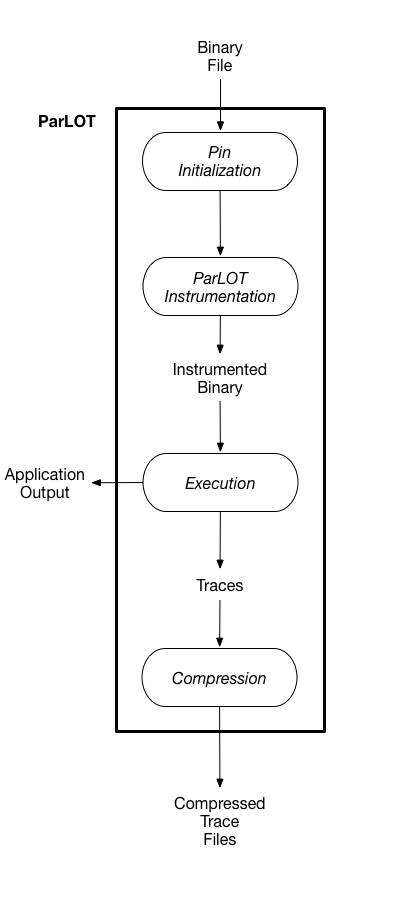
\includegraphics[width=3.5in,height=5in]{figs.chpc/overview.png}
\caption{Overview of ParLOT}
\label{overview}
\end{figure}


\begin{figure}[!t]
\centering
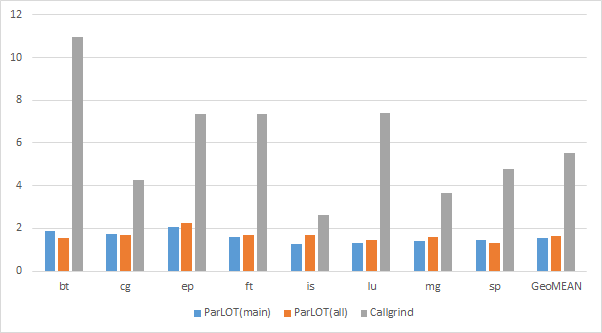
\includegraphics[width=3.5in]{figs.stampede/sd_pin_cg.png}
\caption{Average slowdown of ParLOT(main and all) and Callgrind for 16, 64, and 256 processes. This chart and table \ref{t_compRatio} shows the advantage of ParLoT over callgrind. The geomean of average slowdowns for both ParLOT(main) (1.56) and ParLOT(all) (1.63) is way smaller than Callgrind (5.51). Callgrind scales better (slowdown decreases with larger number of cores) and ParLOT's overhead slightly increases for larger scales.}
\label{sd_pin_cg}
\end{figure}

\begin{table*}[]
\centering
\label{t_sd.pin.cg}

\caption{Slowdown of ParLOT(main and all) and Callgrind. This table and chart \ref{sd_pin_cg} shows the advantage of ParLoT over callgrind. The geomean of average slowdowns for both ParLOT(main) (1.56) and ParLOT(all) (1.63) is way smaller than Callgrind (5.51). Callgrind scales better (slowdown decreases with larger number of cores) and ParLOT's overhead slightly increases for larger scales.}

\begin{tabular}{c|rrrr|rrrr|rrrr|}
\cline{2-13}
\multicolumn{1}{l|}{} & \multicolumn{4}{c|}{ParLOT(main)} & \multicolumn{4}{c|}{ParLOT(all)} & \multicolumn{4}{c|}{Callgrind} \\ \cline{2-13} 
\multicolumn{1}{l|}{} & \multicolumn{1}{c}{16} & \multicolumn{1}{c}{64} & \multicolumn{1}{c}{256} & \multicolumn{1}{c|}{Avg} & \multicolumn{1}{c}{16} & \multicolumn{1}{c}{64} & \multicolumn{1}{c}{256} & \multicolumn{1}{c|}{Avg} & \multicolumn{1}{c}{16} & \multicolumn{1}{c}{64} & \multicolumn{1}{c}{256} & \multicolumn{1}{c|}{Avg} \\ \hline
\multicolumn{1}{|c|}{bt} & 1.63 & 1.86 & 2.11 & 1.87 & 1.49 & 1.65 & 1.52 & 1.55 & 11.04 & 12.93 & 8.86 & 10.94 \\
\multicolumn{1}{|c|}{cg} & 1.28 & 1.79 & 2.07 & 1.71 & 1.31 & 1.6 & 2.17 & 1.69 & 4.86 & 4.71 & 3.21 & 4.26 \\
\multicolumn{1}{|c|}{ep} & 3.06 & 1.77 & 1.38 & 2.07 & 3.13 & 2.17 & 1.49 & 2.26 & 12.95 & 6.08 & 2.99 & 7.34 \\
\multicolumn{1}{|c|}{ft} & 1.69 & 1.47 & 1.69 & 1.62 & 1.71 & 1.62 & 1.69 & 1.67 & 12.04 & 6.48 & 3.58 & 7.37 \\
\multicolumn{1}{|c|}{is} & 1.15 & 1.27 & 1.38 & 1.27 & 1.4 & 1.56 & 2.06 & 1.67 & 2.51 & 1.98 & 3.38 & 2.62 \\
\multicolumn{1}{|c|}{lu} & 1.19 & 1.28 & 1.42 & 1.30 & 1.22 & 1.36 & 1.76 & 1.45 & 7.79 & 7.15 & 7.3 & 7.41 \\
\multicolumn{1}{|c|}{mg} & 1.27 & 1.41 & 1.49 & 1.39 & 1.43 & 1.66 & 1.67 & 1.59 & 4.99 & 3.33 & 2.64 & 3.65 \\
\multicolumn{1}{|c|}{sp} & 1.13 & 1.28 & 1.91 & 1.44 & 1.08 & 1.4 & 1.51 & 1.33 & 3.85 & 6.1 & 4.32 & 4.76 \\ \hline
\multicolumn{1}{|c|}{GeoMean} & 1.46 & 1.50 & 1.66 & \textbf{1.56} & 1.51 & 1.61 & 1.72 & \textbf{1.63} & 6.49 & 5.37 & 4.14 & \textbf{5.51} \\ \hline
\end{tabular}

\end{table*}

\begin{table*}[]
\centering
\label{t_ts.cg}

\caption{Trace bandwidth (kB/s) per core. Average trace bandwidth per core (kB/s) for ParLOT and Callgrind. ParLOT(main) collects very similar call-graph to what Callgrind collects and the average bandwidth required for ParLOT(main) \textbf{4.22} is less half of Callgrind \textbf{8.62}. Also the rate of increasing bandwidth per core for Callgrind is almost twice as ParLOT(look at the \text under line numbers in the table).}

\begin{tabular}{|
>{\columncolor[HTML]{FFFFFF}}c |
>{\columncolor[HTML]{FFFFFF}}r 
>{\columncolor[HTML]{FFFFFF}}r 
>{\columncolor[HTML]{FFFFFF}}r |
>{\columncolor[HTML]{FFFFFF}}r |
>{\columncolor[HTML]{FFFFFF}}r 
>{\columncolor[HTML]{FFFFFF}}r 
>{\columncolor[HTML]{FFFFFF}}r |
>{\columncolor[HTML]{FFFFFF}}r |
>{\columncolor[HTML]{FFFFFF}}r 
>{\columncolor[HTML]{FFFFFF}}r 
>{\columncolor[HTML]{FFFFFF}}r |
>{\columncolor[HTML]{FFFFFF}}r |}
\hline
TOOL & \multicolumn{4}{c|}{\cellcolor[HTML]{FFFFFF}ParLOT(main)} & \multicolumn{4}{c|}{\cellcolor[HTML]{FFFFFF}ParLOT(all)} & \multicolumn{4}{c|}{\cellcolor[HTML]{FFFFFF}Callgrind} \\ \hline
cores & \multicolumn{1}{c}{\cellcolor[HTML]{FFFFFF}16} & \multicolumn{1}{c}{\cellcolor[HTML]{FFFFFF}64} & \multicolumn{1}{c|}{\cellcolor[HTML]{FFFFFF}256} & \multicolumn{1}{c|}{\cellcolor[HTML]{FFFFFF}Avg} & \multicolumn{1}{c}{\cellcolor[HTML]{FFFFFF}16} & \multicolumn{1}{c}{\cellcolor[HTML]{FFFFFF}64} & \multicolumn{1}{c|}{\cellcolor[HTML]{FFFFFF}256} & \multicolumn{1}{c|}{\cellcolor[HTML]{FFFFFF}Avg} & \multicolumn{1}{c}{\cellcolor[HTML]{FFFFFF}16} & \multicolumn{1}{c}{\cellcolor[HTML]{FFFFFF}64} & \multicolumn{1}{c|}{\cellcolor[HTML]{FFFFFF}256} & \multicolumn{1}{c|}{\cellcolor[HTML]{FFFFFF}Avg} \\ \hline
bt & 0.89 & 4.86 & 7.33 & 4.36 & 10.97 & 36.97 & 55.44 & 34.46 & 0.35 & 2.44 & 5.51 & 2.44 \\
cg & 0.50 & 10.58 & 15.17 & 8.75 & 35.30 & 62.26 & 71.75 & 56.44 & 3.63 & 10.49 & 17.69 & 10.49 \\
ep & 2.24 & 1.59 & 0.85 & 1.56 & 15.29 & 25.85 & 32.86 & 24.67 & 2.27 & 12.80 & 26.65 & 12.80 \\
ft & 0.93 & 1.81 & 4.75 & 2.50 & 14.62 & 32.37 & 52.82 & 33.27 & 1.25 & 7.35 & 15.33 & 7.35 \\
is & 0.21 & 1.14 & 1.81 & 1.05 & 45.31 & 42.99 & 35.53 & 41.28 & 21.44 & 30.61 & 24.96 & 30.61 \\
lu & 0.91 & 21.39 & 29.24 & 17.18 & 21.51 & 56.75 & 72.97 & 50.41 & 0.76 & 3.96 & 8.00 & 3.96 \\
mg & 1.84 & 4.86 & 4.69 & 3.80 & 39.1 & 45.13 & 49.31 & 44.51 & 7.66 & 24.89 & 41.66 & 24.89 \\
sp & 0.6 & 11.84 & 17.35 & 9.93 & 12.59 & 46.64 & 99.28 & 52.84 & 0.82 & 4.19 & 8.54 & 4.19 \\ \hline
GeoMean & 0.82 & \underline{4.61} & \underline{4.73} & \textbf{4.22} & 21.25 & 42.11 & 55.31 & \textbf{40.89} & \underline{2.09} & \underline{8.62} & \underline{15.19} & \textbf{8.62} \\ \hline
\end{tabular}
\end{table*}


\begin{table*}[]
\centering
\label{t_overhead}
\caption{\textbf{npin}: Every phase of ParLOT is disabled except Pin-Init (fig \ref{overview}) in \textit{npin} and it shows the pure overhead added by Pin. 
\textbf{wpin}: Compression is disabled in \textit{wpin} and all collected data would be stored as is to the disk. The results of this tools shows how much efficiency our compression approach adds to ParLOT. 
\textbf{dpin}: It is almost identical to ParLOT except it stores the generated compressed traces to "/dev/null". The purpose of \textit{dpin} is to see how much of the overall overhead is because of I/O.
Last row of the table \ref{t-pin-det} shows the average overhead that each of above testing tools adds to the native execution. For each configuration, the differences between the average slowdown of dpin and pin is very insignificant which shows that ParLOT is not an I/O-bounded tool. 
Capturing, collecting and storing the data using ParLOT but without any compression, would cause up to more than 130X slowdown. Again it is another proof for the efficiency that our compression method within ParLOT provides for tracing.}



\begin{tabular}{|c|c|rrrr|rrrr|rrrr|}
\hline
\multicolumn{1}{|l|}{\multirow{2}{*}{}} & Cores & \multicolumn{4}{c|}{16} & \multicolumn{4}{c|}{64} & \multicolumn{4}{c|}{256} \\ \cline{2-14} 
\multicolumn{1}{|l|}{} & Tools & \multicolumn{1}{c}{npin} & \multicolumn{1}{c}{dpin} & \multicolumn{1}{c}{ParLOT} & \multicolumn{1}{c|}{wpin} & \multicolumn{1}{c}{npin} & \multicolumn{1}{c}{dpin} & \multicolumn{1}{c}{ParLOT} & \multicolumn{1}{c|}{wpin} & \multicolumn{1}{c}{npin} & \multicolumn{1}{c}{dpin} & \multicolumn{1}{c}{ParLOT} & \multicolumn{1}{c|}{wpin} \\ \cline{2-14} 
\multirow{8}{*}{Main} & bt & 1.54 & 1.57 & 1.63 & 7.75 & 1.74 & 1.60 & 1.86 & 18.60 & 1.48 & 0.98 & 2.11 & 32.69 \\
 & cg & 1.21 & 1.28 & 1.28 & 1.42 & 1.41 & 1.17 & 1.79 & 43.56 & 1.82 & 1.74 & 2.07 & 73.89 \\
 & ep & 2.18 & 2.76 & 3.06 & 26.91 & 1.63 & 1.69 & 1.77 & 11.65 & 1.24 & 1.08 & 1.38 & 3.40 \\
 & ft & 1.21 & 1.56 & 1.69 & 8.82 & 1.29 & 1.16 & 1.47 & 8.54 & 1.81 & 0.99 & 1.69 & 24.13 \\
 & is & 1.28 & 0.81 & 1.15 & 0.78 & 1.34 & 0.81 & 1.27 & 2.90 & 1.69 & 2.08 & 1.38 & 16.06 \\
 & lu & 1.18 & 1.19 & 1.19 & 1.22 & 1.30 & 1.42 & 1.28 & 10.21 & 1.62 & 1.33 & 1.42 & 34.29 \\
 & mg & 1.26 & 1.05 & 1.27 & 1.20 & 1.39 & 0.98 & 1.41 & 15.97 & 1.38 & 0.89 & 1.49 & 23.76 \\
 & sp & 1.06 & 1.03 & 1.13 & 1.57 & 1.25 & 1.12 & 1.28 & 16.62 & 1.39 & 1.11 & 1.91 & 52.31 \\ \hline
\multicolumn{2}{|c|}{GeoMean} & \textbf{1.33} & \textbf{1.32} & \textbf{1.46} & \textbf{2.88} & \textbf{1.41} & \textbf{1.21} & \textbf{1.50} & \textbf{12.60} & \textbf{1.54} & \textbf{1.27} & \textbf{1.66} & \textbf{24.63} \\ \hline
\multirow{8}{*}{All} & bt & 1.56 & 1.45 & 1.49 & 8.00 & 1.67 & 1.47 & 1.65 & 20.48 & 1.36 & 1.10 & 1.52 & 39.70 \\
 & cg & 1.27 & 1.17 & 1.31 & 2.15 & 1.52 & 1.20 & 1.60 & 49.62 & 2.02 & 1.37 & 2.17 & 83.40 \\
 & ep & 2.31 & 2.89 & 3.13 & 26.96 & 1.77 & 1.61 & 2.17 & 9.92 & 1.34 & 0.96 & 1.49 & 3.33 \\
 & ft & 1.28 & 1.56 & 1.71 & 8.85 & 1.41 & 1.30 & 1.62 & 9.00 & 1.58 & 1.17 & 1.69 & 28.11 \\
 & is & 1.47 & 1.10 & 1.40 & 1.36 & 1.53 & 1.04 & 1.56 & 2.87 & 1.94 & 1.12 & 2.06 & 16.53 \\
 & lu & 1.21 & 1.17 & 1.22 & 2.65 & 1.36 & 1.21 & 1.36 & 11.91 & 1.60 & 1.21 & 1.76 & 42.06 \\
 & mg & 1.41 & 1.22 & 1.43 & 2.15 & 1.56 & 1.15 & 1.66 & 17.24 & 1.66 & 1.27 & 1.67 & 24.70 \\
 & sp & 1.08 & 1.10 & 1.08 & 2.65 & 1.32 & 1.16 & 1.40 & 19.58 & 1.60 & 1.22 & 1.51 & 59.47 \\ \hline
\multicolumn{2}{|c|}{GeoMean} & \textbf{1.41} & \textbf{1.38} & \textbf{1.51} & \textbf{4.13} & \textbf{1.51} & \textbf{1.26} & \textbf{1.61} & \textbf{13.41} & \textbf{1.62} & \textbf{1.17} & \textbf{1.72} & \textbf{27.39} \\ \hline
\end{tabular}
\end{table*}







\begin{figure}[!t]
\centering
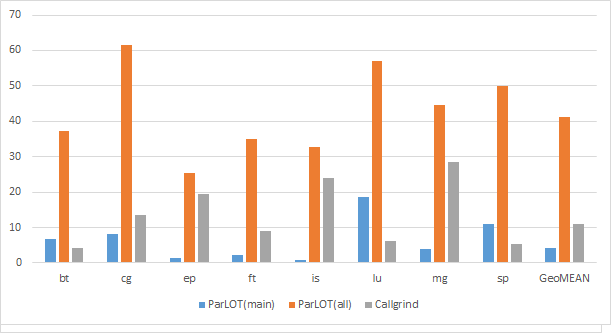
\includegraphics[width=3.5in]{figs.stampede/ts.png}
\caption{Average trace bandwidth per core (kB/s) for ParLOT and Callgrind. ParLOT(main) collects very similar call-graph to what Callgrind collects and the average bandwidth required for ParLOT(main) \textbf{4.22} is less half of Callgrind \textbf{8.62}. Also the rate of increasing bandwidth per core for Callgrind is almost twice as ParLOT(look at the \text under line numbers in the table).  }
\label{ts}
\end{figure}

\begin{figure}[!t]
\centering
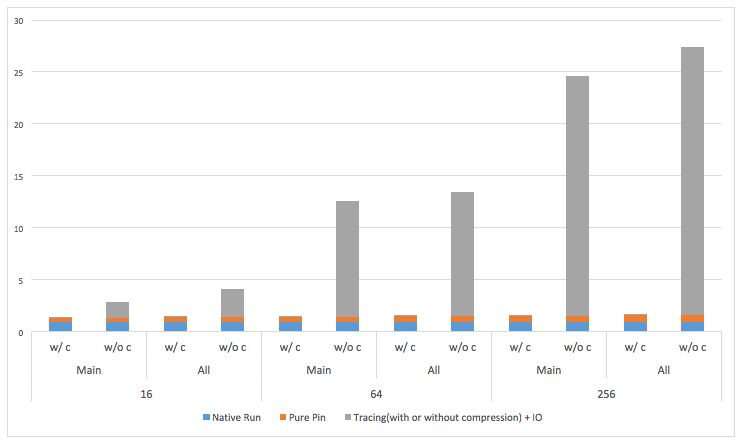
\includegraphics[width=3.5in]{figs.stampede/overhead.png}
\caption{
Average overhead added to the NPB applications by ParLOT, with and without compression. Shows the high impact of compression. This chart is a summary of Table \ref{t_overhead}. }
\label{overhead}
\end{figure}

\begin{figure}[!t]
\centering
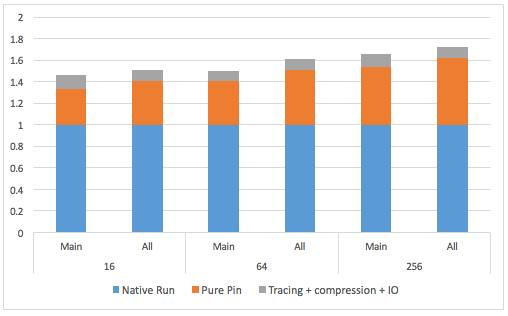
\includegraphics[width=3.5in]{figs.stampede/overhead2.png}
\caption{
(this table is subset of fig \ref{overhead}. Fig \ref{overhead} focuses on the impact of compression and this fig focuses on the overall )
Average overhead added to the NPB applications by ParLOT, I believe this chart shows the low efficiency of ParLOT idea. PIN is considered as \textbf(light-weight) binary instrumentation framework and when you compare the overhead added by Pin and our approach, it is impressive.}
\label{overhead2}
\end{figure}


\begin{table}[]
\centering
\label{t_compRatio}
\caption{This table shows the average ParLOT compression ratios for different NAS applications from the generated traces. For column \textbf{ep} the ratio is high up to 16k. }

\begin{tabular}{ccrrrrrrrr|r|}
\hline
\multicolumn{2}{|c|}{} & \multicolumn{1}{c}{bt} & \multicolumn{1}{c}{cg} & \multicolumn{1}{c}{ep} & \multicolumn{1}{c}{ft} & \multicolumn{1}{c}{is} & \multicolumn{1}{c}{lu} & \multicolumn{1}{c}{mg} & \multicolumn{1}{c|}{sp} & \multicolumn{1}{c|}{GeoMean} \\ \hline
\multicolumn{1}{|c|}{\multirow{3}{*}{Main}} & \multicolumn{1}{c|}{16} & 13895.02 & 5069.90 & 16851.22 & 21035.00 & 50.61 & 418.89 & 344.30 & 3035.00 & 2202.21 \\
\multicolumn{1}{|c|}{} & \multicolumn{1}{c|}{64} & 2157.98 & 339.99 & 15867.32 & 6512.02 & 755.23 & 109.59 & 247.08 & 447.49 & 955.32 \\
\multicolumn{1}{|c|}{} & \multicolumn{1}{c|}{256} & 1742.45 & 261.08 & 14264.38 & 1329.09 & 1176.63 & 166.81 & 484.99 & 295.08 & 837.60 \\ \hline
\multicolumn{1}{|c|}{\multirow{3}{*}{All}} & \multicolumn{1}{c|}{16} & 2186.68 & 161.18 & 9522.48 & 5501.74 & 256.13 & 501.60 & 248.08 & 789.60 & 908.65 \\
\multicolumn{1}{|c|}{} & \multicolumn{1}{c|}{64} & 573.47 & 178.04 & 4043.44 & 1158.27 & 291.89 & 243.27 & 233.64 & 308.42 & 471.60 \\
\multicolumn{1}{|c|}{} & \multicolumn{1}{c|}{256} & 598.73 & 351.75 & 1937.89 & 436.18 & 617.08 & 421.28 & 359.26 & 207.67 & 492.34 \\ \hline 
\end{tabular}
\end{table}


\begin{figure}[!t]
\centering
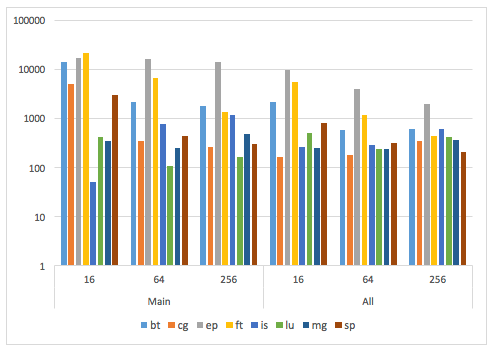
\includegraphics[width=3.5in]{figs.stampede/compRatio.png}
\caption{Compression ratio}
\label{compRatio}
\end{figure}